\documentclass[12pt,a4paper]{article}
\usepackage{cmap} % Makes the PDF copiable. See http://tex.stackexchange.com/a/64198/25761
\usepackage[T1]{fontenc}
\usepackage[brazil]{babel}
\usepackage[utf8]{inputenc}
\usepackage{amsmath}
\usepackage{amsfonts}
\usepackage{amssymb}
\usepackage{amsthm}
\usepackage{textcomp} % \degree
\usepackage{gensymb} % \degree
\usepackage[usenames,svgnames,dvipsnames]{xcolor}
\usepackage{hyperref}
\usepackage{multicol}
\usepackage{graphicx}
\usepackage[margin=2cm]{geometry}

\hypersetup{
    colorlinks = true,
    allcolors = {blue}
}
\usepackage{cancel}

% TODO: Consider using exsheets
% http://linorg.usp.br/CTAN/macros/latex/contrib/exsheets/exsheets_en.pdf
%
% http://ctan.org/tex-archive/macros/latex/contrib/exercise/
% Options: answerdelayed,lastexercise,noanswer
\usepackage[answerdelayed,lastexercise]{exercise}

\addto\captionsbrazil{%
\def\listexercisename{Lista de exerc\'icios}%
\def\ExerciseName{Exerc\'icio}%
\def\AnswerName{Solu\c{c}\~ao do exerc\'icio}%
\def\ExerciseListName{Ex.}%
\def\AnswerListName{Solu\c{c}\~ao}%
\def\ExePartName{Parte}%
\def\ArticleOf{de\ }%
}

\renewcommand{\ExerciseHeaderTitle}{(\ExerciseTitle)\ }
\renewcommand{\ExerciseListHeader}{%\ExerciseHeaderDifficulty%
\textbf{%\ExerciseListName\
\ExerciseHeaderNB.\ %
%\ --- \ 
\ExerciseHeaderTitle}%
%\ExerciseHeaderOrigin
\ignorespaces}
\renewcommand{\AnswerListHeader}{\textbf{\ExerciseHeaderNB.\ (\AnswerListName)\ }}

\newcommand*\sen{\operatorname{sen}}
\newcommand*\tg{\operatorname{tg}}
\newcommand*\R{\mathbb{R}}

\renewcommand{\theenumi}{\alph{enumi}}
\renewcommand\labelenumi{(\theenumi) }

\newcommand*\tipo{Prova II}
\newcommand*\turma{TADS121-01C}
\newcommand*\disciplina{CDI0001}
\newcommand*\eu{Helder G. G. de Lima}
\newcommand*\data{20/03/2017}

\author{\eu}
\title{\tipo - \disciplina}
\date{\data}

\begin{document}
\thispagestyle{empty}
\newgeometry{margin=2cm,bottom=0.5cm}
\begin{center}

\includegraphics[width=9.0cm]{marca} \\
\textbf{\tipo\ (\disciplina / \turma)} \\
Prof. \eu\footnote{
Este é um material de acesso livre distribuído sob os termos da licença \href{https://creativecommons.org/licenses/by-sa/4.0/deed.pt_BR}{Creative Commons BY-SA 4.0}}
\end{center}

\noindent Nome do(a) aluno(a): \underline{\hspace{9,7cm}} Data: \underline{\data}

\begin{center}\fbox{
\begin{minipage}{14cm}

{\footnotesize
\begin{itemize}
\renewcommand{\theenumi}{\Roman{enumi}}
\item Identifique-se em todas as folhas.
\item Mantenha o celular e os demais equipamentos eletrônicos desligados durante a prova.
\item Justifique cada resposta com cálculos ou argumentos baseados na teoria estudada.
\item Resolva apenas os itens de que precisar para somar 10,0 pontos.
\end{itemize}
}

\end{minipage}
}
\end{center}

\begin{ExerciseList}
\Exercise
Considere a função $f: \R_+^* \to \R_+^*$ dada por $f(x) = \frac{4}{\sqrt{x}}$, representada na figura a seguir.
\begin{center}
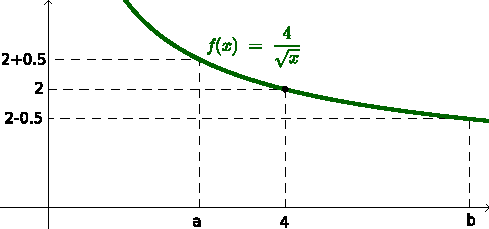
\includegraphics[width=10.9cm]{img/prova-2-tads-limite-def}
\end{center}
\begin{enumerate}
\item \textbf{(1,0)} Obtenha evidências numéricas (use a calculadora se preciso) de qual deve ser o limite de $f$ se $x$ tende a $+\infty$. Confirme o resultado calculando o limite detalhadamente.
\item \textbf{(0,5)} Calcule os valores de $a$ e $b$ indicados na figura.
\item \textbf{(0,5)} Obtenha um número $\delta > 0$ tal que $\left|\frac{4}{\sqrt{x}} - 2 \right| < 0,5$ sempre que $|x-4| < \delta$.
\end{enumerate}

\Answer
\begin{enumerate}
\item Escolhendo valores progressivamente maiores de $x$ obtém-se:
\begin{center}
\begin{tabular}{|c|c|c|c|c|c|c|c|}
\hline
$x$    & 100 & 400 & 2500 & 10000 & 1000000 & 100000000 \\
\hline
$f(x)$ & 0.4 & 0.2 & 0.08 &  0.04 &   0.004 & 0.0004 \\
\hline
\end{tabular}
\end{center}
Como os valores de $f(x)$ estão cada vez mais próximos de zero, isso sugere que $\frac{4}{\sqrt{x}} \to 0$ quando $x \to +\infty$. De fato, pelas propriedades de limite, resulta que:
\[
\lim_{x \to +\infty} \frac{4}{\sqrt{x}}
= \lim_{u \to +\infty} \frac{4}{u}
= \lim_{t \to 0^+} 4 t
= 4 \cdot \lim_{t \to 0^+} t
= 4 \cdot 0
= 0.
\]
\item Tem-se:
\[
f(a) =
\frac{4}{\sqrt{a}} = 2.5 = \frac{5}{2}
\Leftrightarrow
\sqrt{a} = \frac{4}{2.5} = \frac{8}{5}
\Leftrightarrow
a = \left( \frac{4}{2.5} \right)^2 = \frac{64}{25} = 2,56
\]
e
\[
f(b) =
\frac{4}{\sqrt{a}} = 1.5 = \frac{3}{2}
\Leftrightarrow
\sqrt{a} = \frac{4}{1.5} = \frac{8}{3}
\Leftrightarrow
b = \left( \frac{4}{1.5} \right)^2 = \frac{64}{9} = 7,1\overline{1}.
\]

\item Pelo item anterior, basta escolher a $\delta$ como a menor distância entre $4$ e $a$ e $b$, isto é,
\[
\delta
= \min\{ 4-a, b-4 \}
= \min\left\{ 4-\frac{64}{25}, \frac{64}{9}-4 \right\}
= \min\left\{ \frac{36}{25}, \frac{28}{9} \right\}
= \frac{36}{25}
= 1,44.
\]

De fato, pode-se verificar essa afirmação observando que
$|x-4| < \frac{36}{25}
\Leftrightarrow
4 - \frac{36}{25} < x < 4 + \frac{36}{25}$,
pois como $\frac{36}{25} < \frac{28}{9}$, tem-se que:
\begin{align*}
|x-4| < \frac{36}{25}
& \Rightarrow
4 - \frac{36}{25} < x < 4 + \frac{28}{9}
\Leftrightarrow
\frac{64}{25} < x < \frac{64}{9}
\Leftrightarrow
\frac{8}{5} < \sqrt{x} < \frac{8}{3}\\
& \Leftrightarrow
\frac{2}{5} < \frac{ \sqrt{x} }{4} < \frac{2}{3}
\Leftrightarrow
\frac{3}{2} < \frac{ 4 }{\sqrt{x}} < \frac{5}{2}
\Leftrightarrow
\frac{3}{2} - 2 < \frac{ 4 }{\sqrt{x}} - 2 < \frac{5}{2} - 2\\
& \Leftrightarrow
-\frac{1}{2} < \frac{ 4 }{\sqrt{x}} - 2 < \frac{1}{2}
\Leftrightarrow
\left| \frac{ 4 }{\sqrt{x}} - 2 \right| < \frac{1}{2}.
\end{align*}
\end{enumerate}

\Exercise[title={2,0}] Determine $A$ e $B$ para que seja contínua a função
$
g(x) =
\begin{cases}
\frac{x^2 + x}{x+1}, \text{ se } x < -1,\\
Ax + B, \text{ se } -1 \leq x \leq 0,\\
\frac{e^{4x}-1}{e^{2x}-1}, \text{ se } x > 0.
\end{cases}$
\Answer Para que $g$ seja contínua, ela deve ser contínua em cada ponto $a \in \R$. Para $a \not\in \{-1, 0\}$, $g$ é contínua, pois coincide com uma função afim em $[-1, 0]$, e com quocientes entre funções contínuas em $(-\infty, -1)$ e em $(0, +\infty)$, cujos denominadores não se anulam em $(-\infty, -1) \cup (0, +\infty)$. Assim, resta apenas a análise dos limites em $-1$ e $0$. Tem-se:
\[
\lim_{x \to -1^-} g(x)
= \lim_{x \to -1^-} \frac{x^2 + x}{x+1}
= \lim_{x \to -1^-} \frac{x(x + 1)}{x+1}
= \lim_{x \to -1^-} x
= -1,
\]
\[
\lim_{x \to -1^+} g(x)
= \lim_{x \to -1^-} Ax+B
= B-A = g(-1),
\]
\[
\lim_{x \to 0^+} g(x)
= \lim_{x \to 0^+} \frac{e^{4x}-1}{e^{2x}-1}
= \lim_{x \to 0^+} \frac{ \frac{e^{4x}-1}{x} }
                        { \frac{e^{2x}-1}{x} }
= \lim_{x \to 0^+} \frac{ 4\frac{e^{4x}-1}{4x} }
                        { 2\frac{e^{2x}-1}{2x} }
= 2 \frac{ \lim_{x \to 0^+} \frac{e^{4x}-1}{4x} }
         { \lim_{x \to 0^+} \frac{e^{2x}-1}{2x} }
= 2 \frac{ \lim_{u \to 0^+} \frac{e^{u}-1}{v} }
         { \lim_{v \to 0^+} \frac{e^{v}-1}{v} }
= 2,
\]
(outra alternativa:
$\lim_{x \to 0^+} \frac{e^{4x}-1}{e^{2x}-1}
= \lim_{x \to 0^+} \frac{(e^{2x}-1)(e^{2x}+1)}{e^{2x}-1}
= \lim_{x \to 0^+} e^{2x}+1
= e^0 + 1 = 2$
)
\[
\lim_{x \to 0^-} g(x)
= \lim_{x \to 0^-} Ax+B
= B = g(0).
\]
Assim, para que $g$ seja contínua, $A$ e $B$ devem satisfazer as seguintes condições:
\[
\begin{cases}
B-A & = -1\\ 
B   & = 2
\end{cases}
\]
Portanto, $B = 2$ e $A = 3$.

\Exercise
Uma prática bastante comum em diversos estabelecimentos comerciais é dar descontos aos consumidores na forma de promoções do tipo ``leve 3 pague 2'' ou ``compre 3 pizzas e ganhe 1 grátis''. O comerciante pode escolher livremente a quantidade $n$ de produtos que devem ser comprados, para que seja dado um de graça. Matematicamente, se o cliente levar ``n+1'' produtos pelo preço de ``n'' unidades, receberá um desconto que é calculado por $d(n) = \frac{100}{n+1} \%$.
\begin{enumerate}
\item \textbf{(1,0)} Para que valores de $n$ o cliente recebe menos de $10\%$ de desconto?
\item \textbf{(1,0)} O que ocorre com o desconto se $n$ tende a infinito? Isso é vantajoso para o cliente?
\end{enumerate}

\Answer
\begin{enumerate}
\item Considerando $n > 0$, o desconto é menor do que $10\%$ quando
\[
\frac{100}{n+1} < 10
\Leftrightarrow
100 < 10(n+1)
\Leftrightarrow
100 < 10n + 10
\Leftrightarrow
90 < 10n
\Leftrightarrow
n > 9.
\]

\item Como
\[
\lim_{n \to +\infty} \frac{100}{n+1}
= \lim_{u \to +\infty} \frac{100}{u}
= 100 \lim_{u \to +\infty} \frac{1}{u}
= 100 \cdot 0 = 0,
\]
o desconto tende a ser cada vez menor quando $n \to +\infty$. Logo, o aumento da quantidade $n$ não é vantajoso para o cliente (mas sim para o comerciante), pois quanto maior é o valor de $n$, menor é o desconto dado:
\[
n_1 < n_2
\Rightarrow
n_1+1 < n_2+1
\Rightarrow
\frac{1}{n_2+1} < \frac{1}{n_1+1}
\Rightarrow
\frac{100}{n_2+1} < \frac{100}{n_1+1}
\Rightarrow
d(n_2) < d(n_1).
\]
\end{enumerate}

\Exercise Calcule os seguintes limites, detalhando todos os passos necessários para obter a resposta:
\begin{multicols}{2}
\begin{enumerate}
\item \textbf{(2,0)} $\displaystyle\lim_{ x \to +\infty } \cos\left(\sqrt{3x-3}-\sqrt{3x}\right) $
\item \textbf{(2,0)} $\displaystyle\lim_{ x \to 0^+ } \ln( \sen(e x) ) - \ln(\tg(x)) $
\item \textbf{(2,0)} $\displaystyle\lim_{ x \to -\infty } \dfrac{ -5x^3 + 4x + 8}{25x^2-3x-2}$
\end{enumerate}
\end{multicols}
\Answer
\begin{enumerate}
\item Considerando que
\begin{align*}
\sqrt{3x-3}-\sqrt{3x}
& = \sqrt{3(x-1)} - \sqrt{3x}
  = \sqrt{3} \cdot
    \left( \sqrt{x - 1} - \sqrt{x}\right)\\
& = \sqrt{3} \cdot
    \left( \sqrt{x - 1} - \sqrt{x}\right) \cdot
    \frac{ \sqrt{x-1}+\sqrt{x} }
         { \sqrt{x-1}+\sqrt{x} }\\
& = \sqrt{3} \cdot
    \frac{ (x - 1) - x }
         { \sqrt{x-1}+\sqrt{x} }
 = \frac{ -\sqrt{3} }
        { \sqrt{x-1}+\sqrt{x} },
\end{align*}
e que $\cos$ é contínua, tem-se
\begin{align*}
\lim_{ x \to +\infty } \cos\left(\sqrt{3x-3}-\sqrt{3x}\right)
& = \cos \left( \lim_{ x \to +\infty }
  \frac{ -\sqrt{3} }
       { \cancelto{+\infty}{\sqrt{x-1}}+\cancelto{+\infty}{\sqrt{x}} } \right) \\
& = \cos \left( \lim_{ t \to +\infty }
  \frac{ -\sqrt{3} }
       { t } \right)
= \cos(0) = 1.
\end{align*}

\item Considerando que
\begin{align*}
\ln( \sen(e x) ) - \ln(\tg(x))
& = \ln\left( \frac{ \sen(e x) }{ \tg(x) }\right)
  = \ln\left(
    \frac{ \sen(e x) }
         { \frac{\sen(x)}{\cos(x)} }\right)
  = \ln\left( \sen(e x) \cdot
    \frac{ \cos(x) }
         { \sen(x) } \right)\\
& = \ln\left(
    \frac{ \sen(e x) }
         { ex } \cdot
    \frac{ ex }
         { \sen(x) } \cdot
    \cos(x) \right)
  = \ln\left(
    \frac{ \sen(e x) }
         { ex } \cdot
    \frac{ e \cos(x) }
         {\frac{ \sen(x) }
               { x }  }
     \right),
\end{align*}
e que $\ln$ é contínua, tem-se
\begin{align*}
\lim_{ x \to 0^+ } \ln( \sen(e x) ) - \ln(\tg(x))
& = \ln\left( \lim_{ x \to 0^+ }
    \frac{ \sen(e x) }
         { ex } \cdot
    \frac{ e \cos(x)}
         {\frac{ \sen(x) }
               { x }  }
    \right) \\
& = \ln\left(
    \lim_{ x \to 0^+ } \frac{ \sen(e x) }
         { ex } \cdot
    \lim_{ x \to 0^+ }
         \frac{ \cancelto{e}{ e \cos(x)} \quad }
              { \cancelto{1}{ \frac{ \sen(x) }
                    { x }} }
     \right) \\
& = \ln\left(
    \lim_{ v \to 0^+ }
         \cancelto{1}{ \frac{ \sen(v) }
                     { v }} \cdot
         \frac{ e }
              { 1 }\right)
  = \ln(e) = 1.
\end{align*}

\item Tem-se
\begin{align*}
\lim_{ x \to -\infty } \dfrac{ -5x^3 + 4x + 8}
                             { 25x^2 - 3x - 2}
& = \lim_{ x \to -\infty }
    \dfrac{ x^2(-5x + 4/x + 8/x^2)}
          { x^2( 25 - 3/x - 2/x^2)} \\
& = \lim_{ x \to -\infty }
    \dfrac{\cancelto{+\infty}{-5x}\qquad+\ \cancelto{0}{4/x + 8/x^2}}
          {\cancelto{25}{25 - 3/x - 2/x^2}}
  = +\infty
\end{align*}
\end{enumerate}
\end{ExerciseList}

\begin{center}
BOA PROVA!
\end{center}

\newpage
\restoregeometry
\section*{Respostas}
\shipoutAnswer
\end{document}
